% !TEX root = ../main.tex

\section{Measurement Setup}
\label{sec:results-setup}

\scaffold{
  \textbf{Paragraph 1, equipment.} Oscilloscope Rigol MSO5104, laboratory supply Rigol DP932E, shown in \cref{fig:measurement-setup}; the ADCs of the board itself serve as the instrument for everything below the oscilloscope's resolution (noise, position), and the firmware logs over the debug probe for rates and state changes. Name the test points used per measurement (\cref{sec:pcb}). Give the supply voltage used for all measurements.
}

\scaffold{
  \textbf{Paragraph 2, a lesson on probes.} The first oscilloscope captures were taken with the probes on 1X. Three independent signs revealed it: floating contacts discharged with a time constant of about \qty{10}{\milli\second} (the \qty{1}{\mega\ohm} input against \qty{10}{\nano\farad}), a contact showed about \qty{150}{\pico\farad} of load, and SPI edges looked like they were driving 100 to \qty{130}{\pico\farad}. All timing and edge measurements were repeated at 10X, which loads the circuit far less \cite{tektronix2026probes}; the supply ripple measurements are taken at 1X on purpose, for the lower noise floor. State this in two sentences as part of the method, not as an apology.
}

\begin{figure}[htbp]
  \centering
  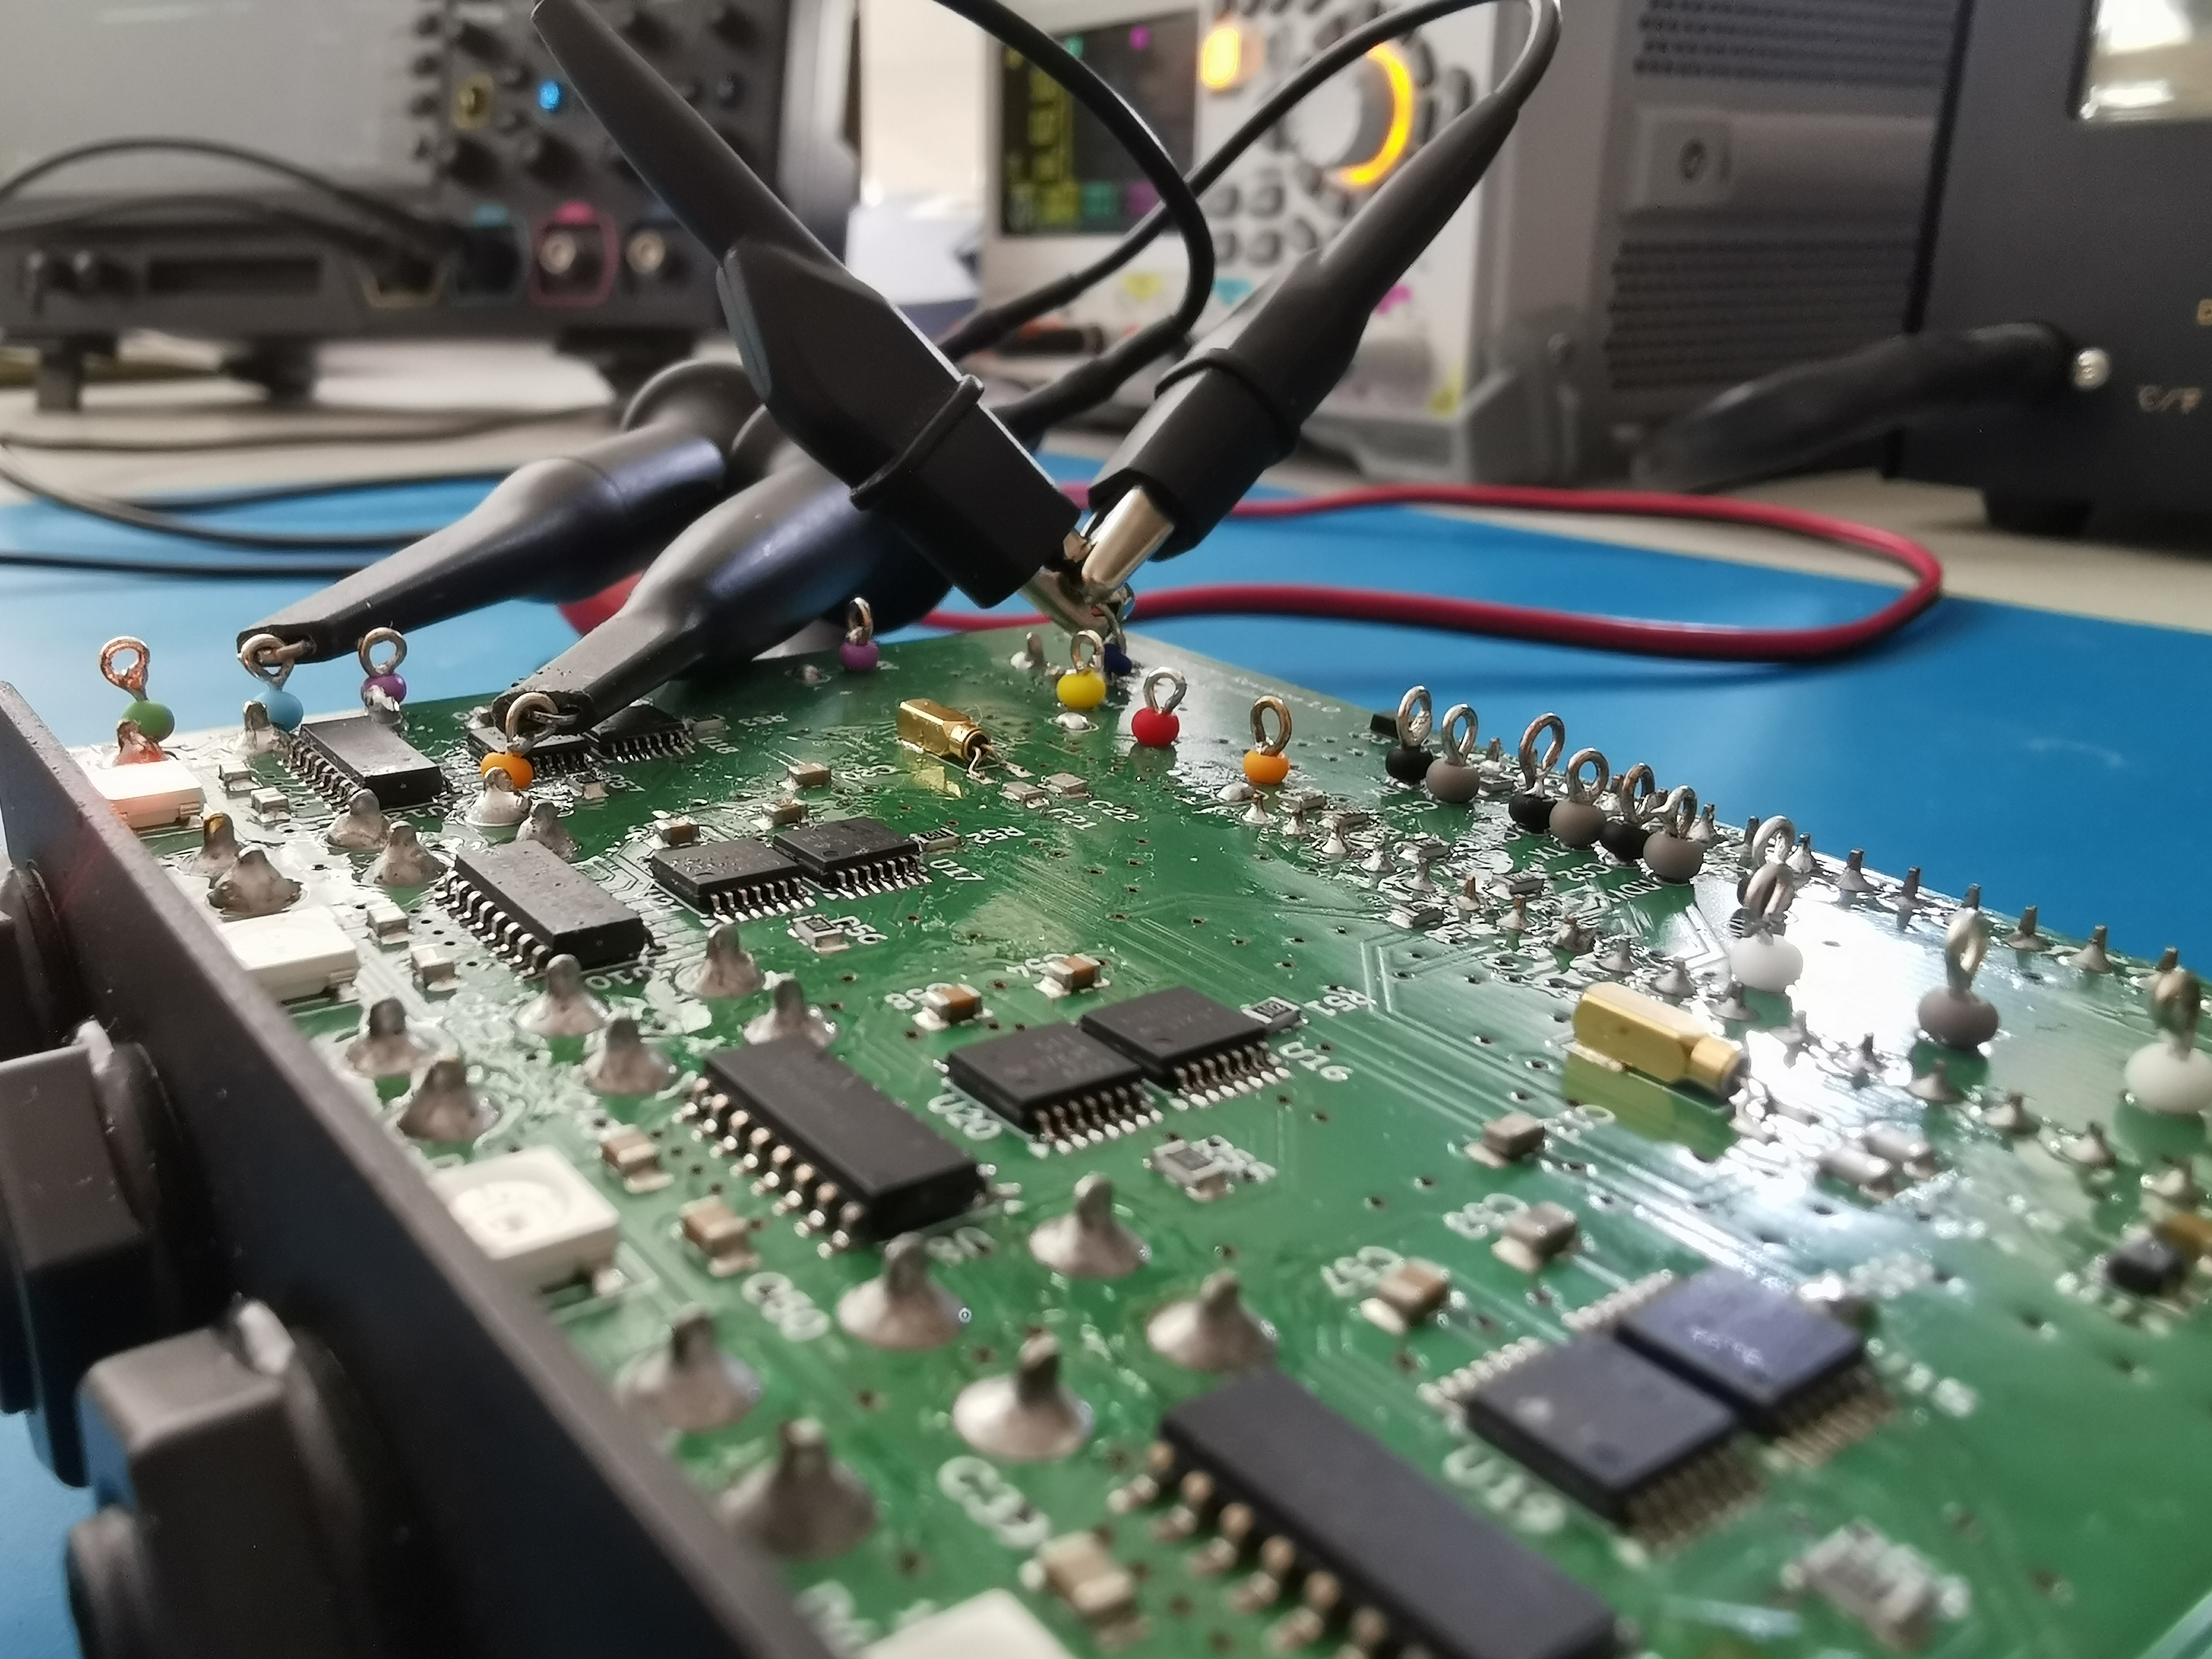
\includegraphics[width=0.75\linewidth]{05-results/figures/measurement-setup}
  \titledcaption{Measurement Setup}{\scaffoldinline{Name the board, the probes and their test points, the pedal and the instruments visible in the photo.}}
  \label{fig:measurement-setup}
\end{figure}

\openquestion{Supply voltage of the measurements}{
  Give the input voltage set on the DP932E for the measurements and the probe model used.
}
